\documentclass[conference]{IEEEtran}
\IEEEoverridecommandlockouts
% The preceding line is only needed to identify funding in the first footnote. If that is unneeded, please comment it out.
\usepackage{cite}
\usepackage{amsmath,amssymb,amsfonts}
\usepackage{algorithmic}
\usepackage{graphicx}
\usepackage{textcomp}
\usepackage{xcolor}
\def\BibTeX{{\rm B\kern-.05em{\sc i\kern-.025em b}\kern-.08em
    T\kern-.1667em\lower.7ex\hbox{E}\kern-.125emX}}
\begin{document}

\title{Signal Processing Approach for Triangle Mesh Smoothing}
\author{\IEEEauthorblockN{Shaoyu Chen}}
\maketitle

\begin{abstract}
In this project, we implemented a signal processing approach for surface signal fairing \cite{taubin1995signal} which overcomes the drawbacks of Laplacian smoothing. Then we compare this approach with the Laplacian smoothing and find that it do outperform the Laplacian smoothing. 
\end{abstract}

\section{Introduction}

The Laplacian smoothing has several drawbacks such as shrinkage and over-smoothing. These drawbacks make the Laplacian smoothing unfeasible in many cases. A signal processing approach for triangle mesh smoothing \cite{taubin1995signal} is proposed to overcome the drawbacks of the Laplacian smoothing.

\section{Methodology}

Define the discrete Laplacian of a vertex $x_i$ by:
\begin{equation}
\Delta x_i = \sum_{j\in i^*}w_{ij}(x_j-x_i)
\end{equation}
where $i^*$ is the set of the first order neighbors of $x_i$, $w_{ij}$ are positive numbers and $\sum_{j\in i^*}w_{ij}=1$.

The $w_{ij}$ is set to $\frac{1}{|i^*|}$ for simplicity and efficiency. Alternatively, a positive function $\phi$ where $\phi(v_i,v_j)=\phi(v_j,v_i)$ can be used and $w_{ij}=\frac{\phi(V_i,v_j)}{\sum_{h\in i^*}\phi(v_i,v_h)}$. One example of such function is $\phi(v_i,v_j)=\frac{1}{\|v_i-v_j\|}$  so that the closer a neighbor is, the larger weight it will have.

After obtaining the discrete Laplacian, for Laplacian smoothing, the position of the vertex $x_i$ is updated by
\begin{equation}
x_i=x_i+\lambda\Delta x_i
\end{equation}
where the $0<\lambda\leq1$ is the scale factor. It is worthwhile to mention that when $\lambda<0$ or $\lambda>1$, this update will enhance high frequencies instead of smoothing.

However, the Laplacian smoothing will lead to the shrinkage of the surface since it is not a low pass filter. To compensate the shrinkage, an un-shrinking step $x_i=x_i+\mu\Delta x_i$ is added after the shrinking step $x_i=x_i+\lambda\Delta x_i$. The $\mu$ is a new negative scale factor such that $\mu<-\lambda$.

The algorithm of one iteration of our approach is showed as follows:
\begin{algorithmic}
	\REQUIRE $x_i$
	\ENSURE $0<\lambda\leq1, \mu<-\lambda$
	\FOR{$i=1$ \TO $N$}
	\STATE 	$\Delta x_i \leftarrow \sum_{j\in i^*}w_{ij}(x_j-x_i)$
	\ENDFOR
	\FOR{$i=1$ \TO $N$}
	\STATE  $x_i\leftarrow x_i+\lambda\Delta x_i$
	\ENDFOR
	\FOR{$i=1$ \TO $N$}
	\STATE 	$\Delta x_i \leftarrow \sum_{j\in i^*}w_{ij}(x_j-x_i)$
	\ENDFOR
	\FOR{$i=1$ \TO $N$}
	\STATE  $x_i\leftarrow x_i+\mu\Delta x_i$
	\ENDFOR
\end{algorithmic}

It is proved that this algorithm is a low pass filter \cite{taubin1995signal} and $k_{pb} = \frac{1}{\lambda}+\frac{1}{\mu}$ is the pass-band frequency of the low pass filter. In the following experiments, $k_{pb}=0.1$ and $\lambda=0.5$.

\section{Results}
Figure \ref{1png} shows an isosurface $f(x,y,z)=0$ where $f(x,y,z)=\cos(x)+\cos(y)+\cos(z)$ and the isosurface corrupted by normal noise. Figure \ref{2png} shows the results after 2 iterations. Both methods can return a smoother surface after 2 iterations. The result of Laplacian smoothing is smoother than the result of signal processing approach since the un-shrinking step slows down the smoothing of signal processing approach. Also, here the shrinkage of Laplacian smoothing is not obvious. Figure \ref{3png} shows the results after 10 iterations, the results of both methods are quite smooth, but we can start to see the shrinkage of Laplacian smoothing since the holes of the surface are larger than those of the original surface. Figure \ref{4png} shows the results after 50 iterations. Compared with the corresponding result after 10 iterations, the result of signal processing approach has a slight improvement while the result of Laplacian smoothing suffers from the shrinkage and over-smoothing.

A square surface, as shown in figure \ref{7png}, is an example where the Laplacian smoothing is not suitable. Figure \ref{5png} shows the result of Laplacian smoothing after 100 iterations. After Laplacian smoothing, the shape of the face is no longer a square. In addition to the change of shape, the coordinates of the four vertices also change significantly and the change indicates that the area of the face is much smaller after smoothing. Figure \ref{6png} shows the result of signal processing approach after 100 iterations. Compared with the original square, the result is almost the same in terms of shape and area.

Figure \ref{8png} shows an example where half of the sphere is corrupted by normal noise. We can see that the signal processing approach smooths the corrupted half while the uncorrupted part is almost unchanged.

\subsection{Discussion}

In the previous examples, we can see that the signal processing approach outperforms the Laplacian smoothing since it can preserve the area and the shape of the original surface. Also, the signal processing approach does not change the smooth part of a surface so it will not suffer from over-smoothing, which is a main drawback of the Laplacian smoothing.

\section{Conclusion}

In experiments we find that the signal processing approach overcomes the drawbacks of Laplacian smoothing. It is also quite simple to implement this approach -- just adding an un-shrinking step after the shrinking step of Laplacian smoothing. For this reason, the signal processing approach has the same time and space complexity as the Laplacian smoothing. Both methods have linear time and space complexity. The reasons above make this signal processing approach a good choice for triangle mesh smoothing.

\begin{figure}
	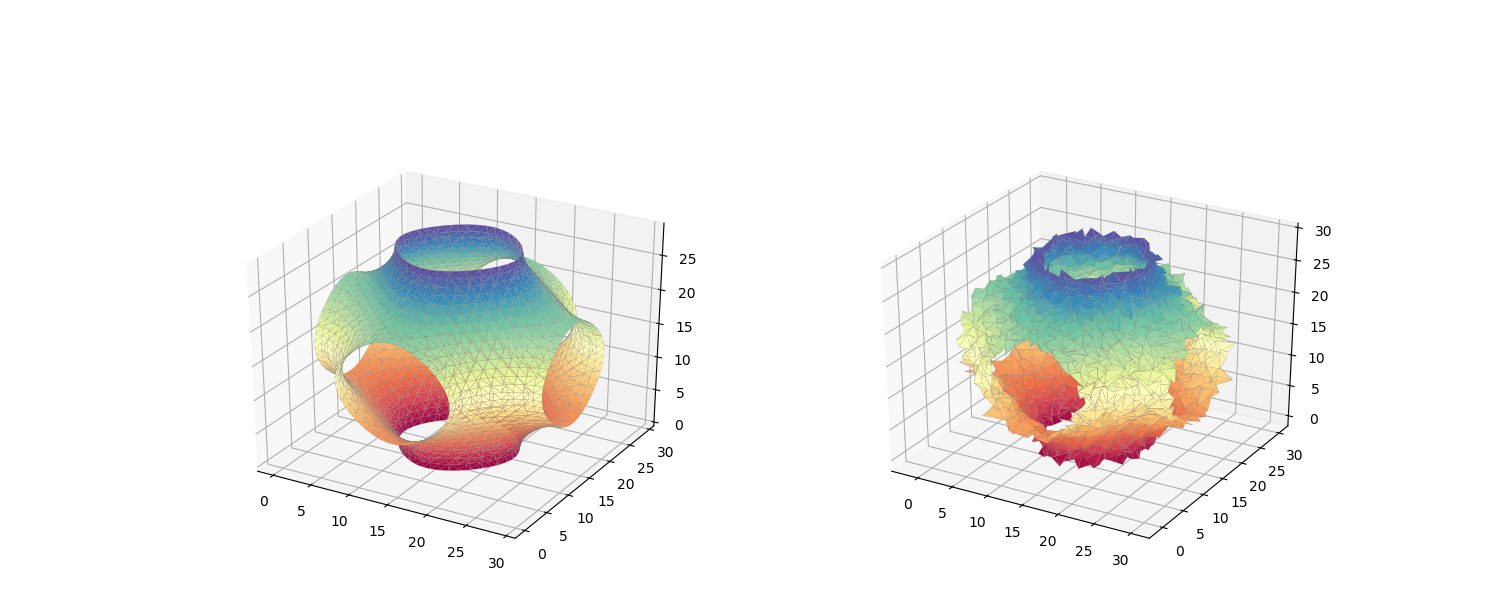
\includegraphics[width=\linewidth]{1.png}
	\caption{Left: original surface \space Right: surface corrupted by normal noise}
	\label{1png}

	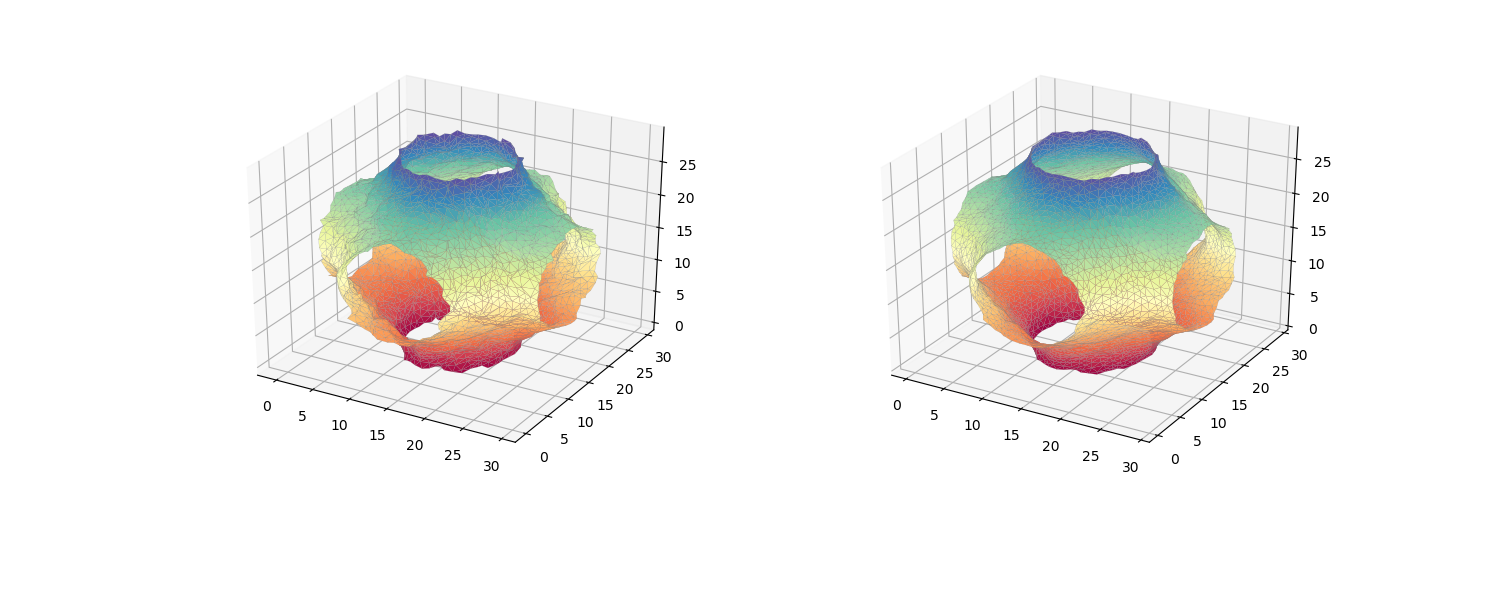
\includegraphics[width=\linewidth]{2.png}
	\caption{Result after 2 iterations \newline Left: signal processing approach \space Right: Laplacian smoothing}
	\label{2png}

	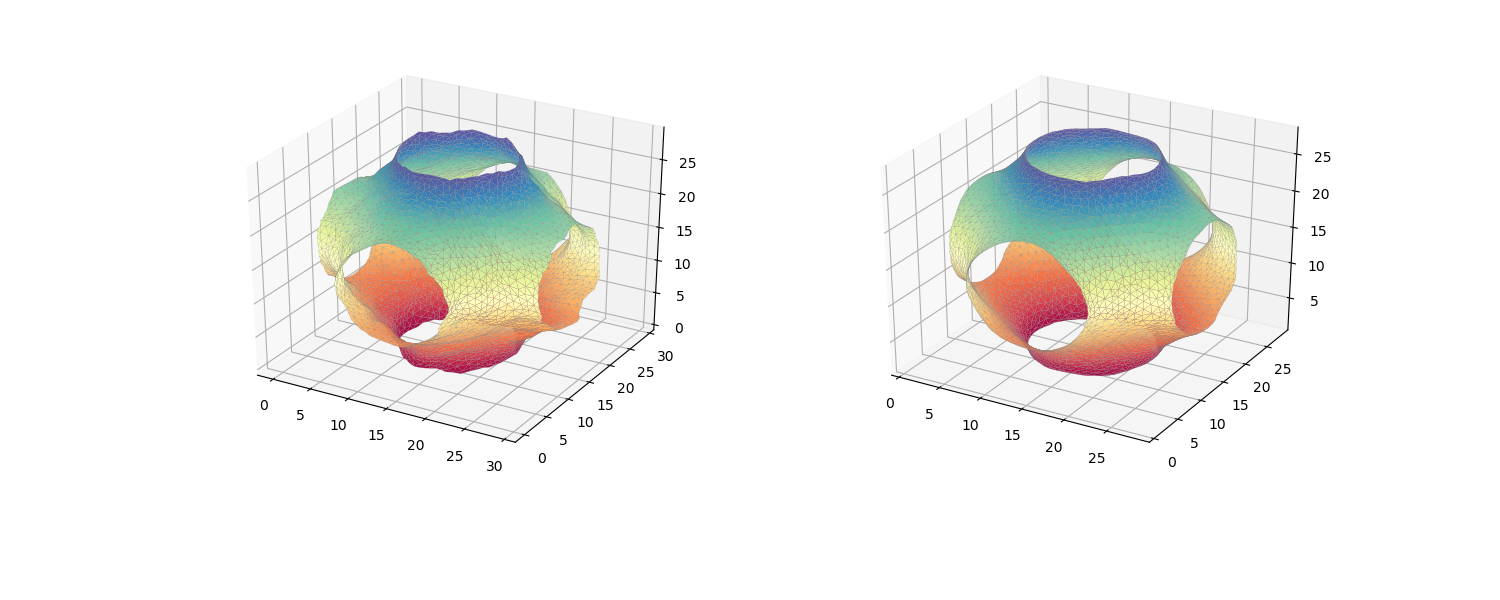
\includegraphics[width=\linewidth]{3.png}
	\caption{Result after 10 iterations \newline Left: signal processing approach \space Right: Laplacian smoothing}
	\label{3png}

	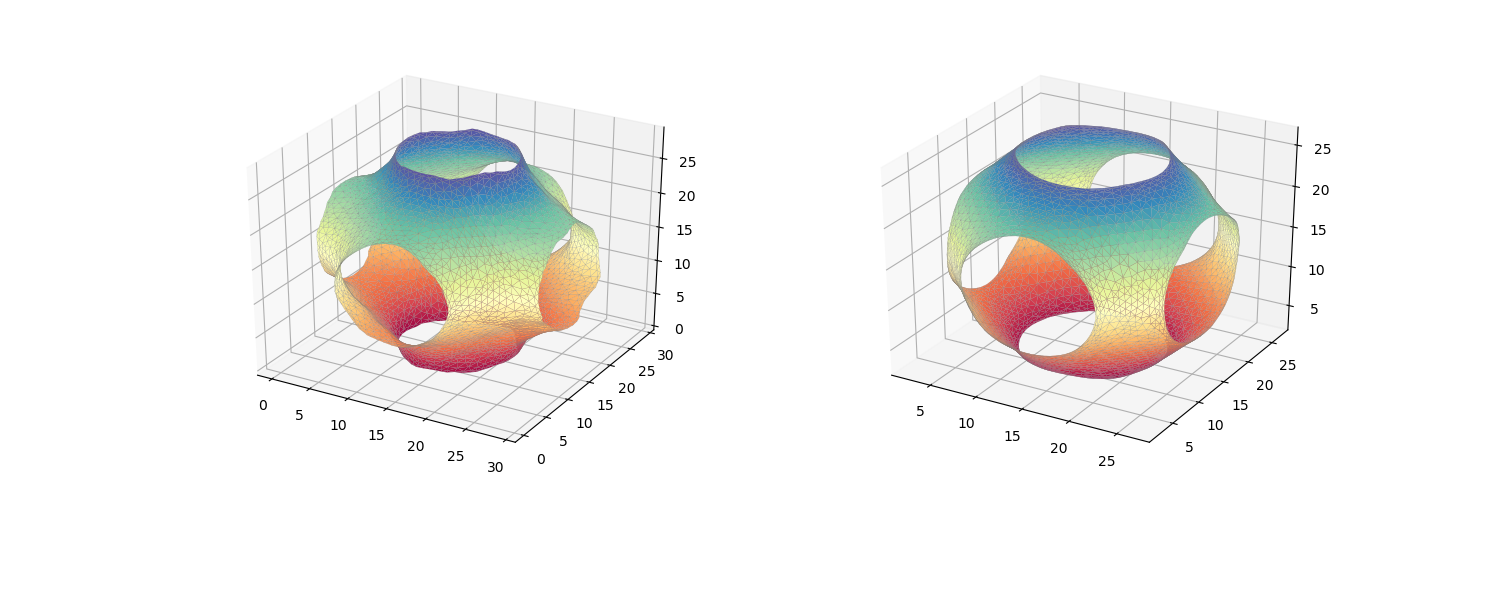
\includegraphics[width=\linewidth]{4.png}
	\caption{Result after 50 iterations \newline Left: signal processing approach \space Right: Laplacian smoothing}
	\label{4png}
\end{figure}
\begin{figure}
	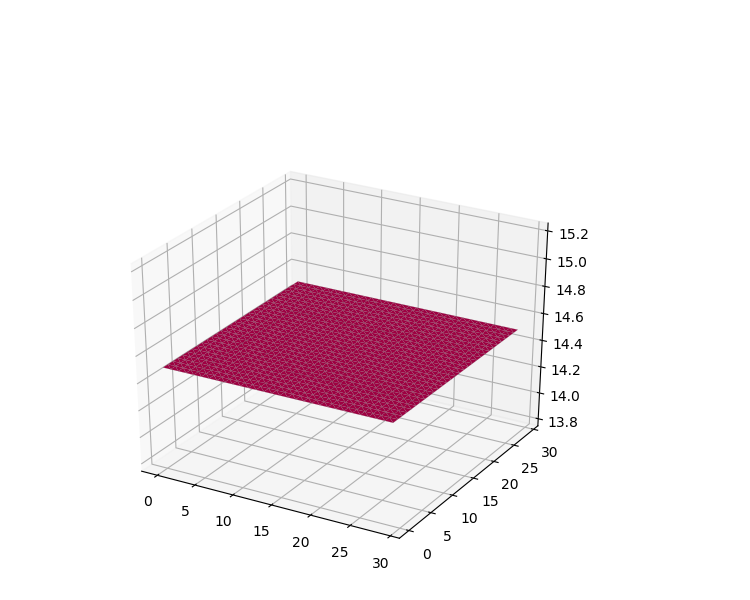
\includegraphics[width=3.5in]{7.png}
	\caption{A square face}
	\label{7png}

	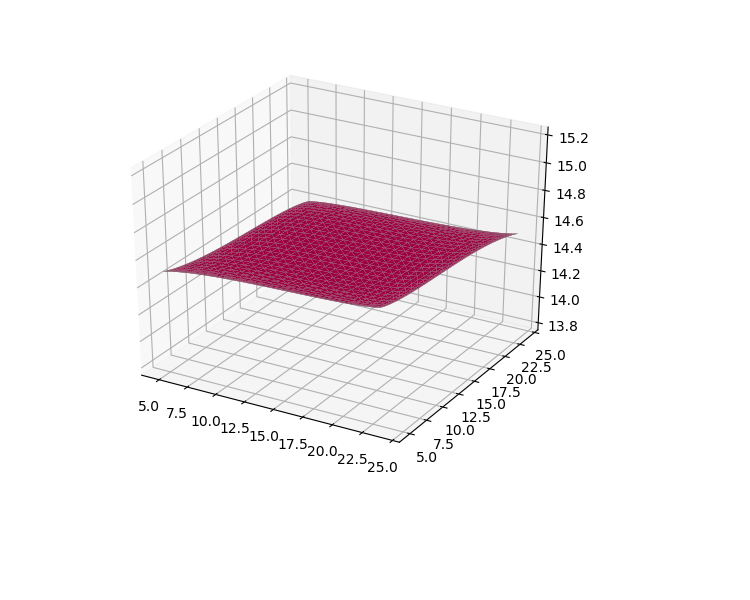
\includegraphics[width=3.5in]{5.png}
	\caption{Result of Laplacian smoothing after 100 iterations}
	\label{5png}

	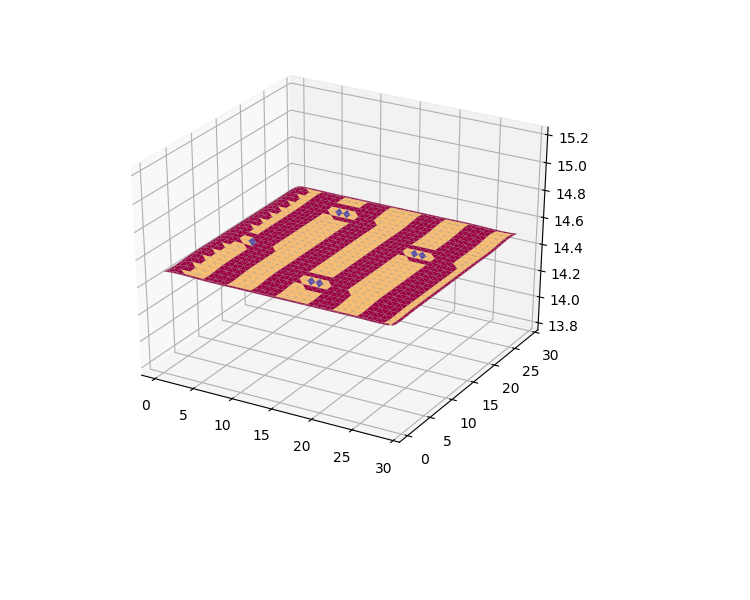
\includegraphics[width=3.5in]{6.png}
	\caption{Result of signal processing approach after 100 iterations}
	\label{6png}
\end{figure}
\begin{figure}
	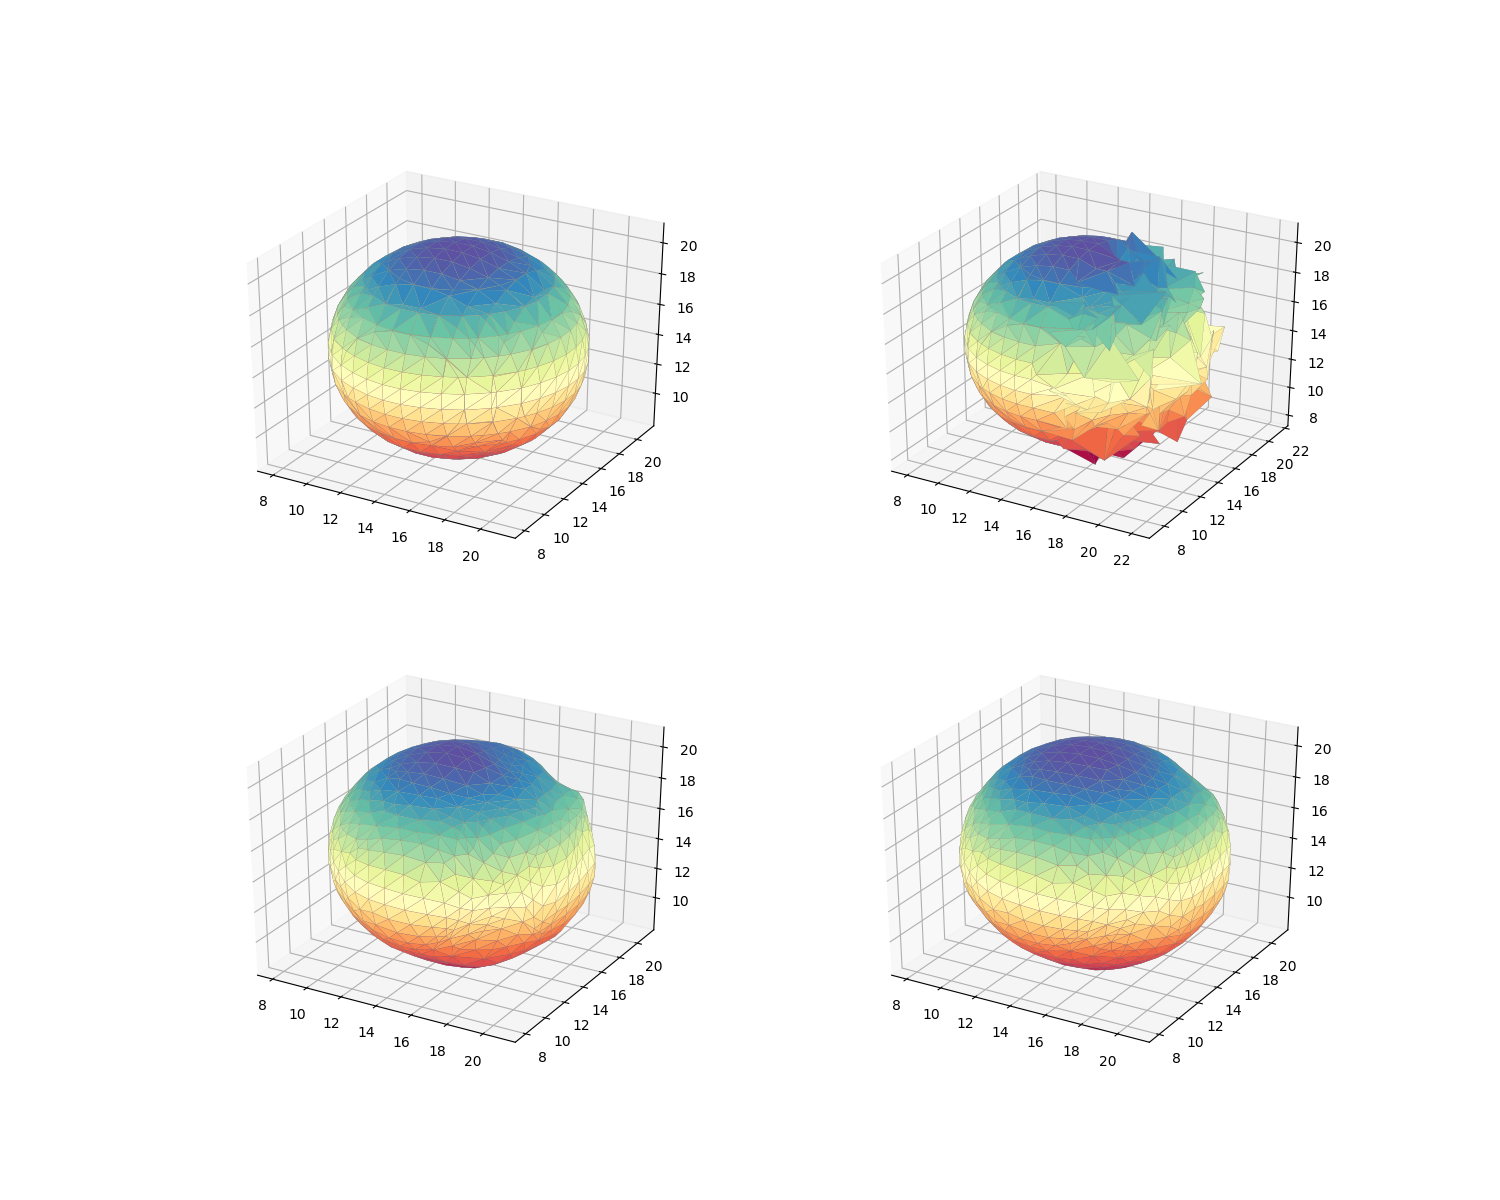
\includegraphics[width=4.2in]{8.png}
	\caption{Top left: original sphere, Top right: sphere partially corrupted by normal noise, Bottom left: result of signal processing approach after 10 iterations, Bottom right: result of signal processing approach after 50 iterations}
	\label{8png}
\end{figure}

\bibliography{ref}
\bibliographystyle{ieeetr}

\end{document}
